\section{Les boucles}
%\leconwithtoc

\subsection{La notion de travail répétitif}

\begin{frame}{La notion de travail répétitif}
	\begin{itemize}
		\item
		Les ordinateurs révèlent tout leur potentiel dans leur capacité à
		répéter inlassablement les mêmes tâches. 
	\item
		Si on veut faire effectuer un travail répétitif, 
		il faut indiquer deux choses~:
		
		\begin{enumerate}
			\item Le travail à répéter
			\item La manière de continuer la répétition 
				ou de l'arrêter.
		\end{enumerate}

	\end{itemize}
\end{frame}

\begin{frame}{Exemple 1}
	Pour traiter des dossiers, on dira quelque chose
	comme «~tant qu'il reste un dossier à traiter, le
	traiter~» ou encore «~traiter un dossier puis passer au suivant
	jusqu'à ce qu'il n'en reste plus à traiter~».

	\begin{itemize}
	\item la tâche à répéter est : «~traiter un dossier~»
	\item on indique qu'on doit continuer s'il
		reste encore un dossier à traiter
	\end{itemize}
	
	\bigskip

	\textbf{Remarque :} On aurait aussi pu le formuler ainsi : «~traiter un
	dossier et passer au suivant jusqu'à ce
	qu'il n'en reste plus~»
\end{frame}

\begin{frame}{Exemple 2}
	Pour calculer la cote finale de tous les étudiants,
	on aura quelque chose du genre «~Pour tout étudiant, calculer sa
	cote~»

	\begin{itemize}
	\item 
		La tâche à répéter est : «~calculer la cote d'un
		étudiant~»
	\item 
		On indique qu'on doit le faire pour tous les étudiants.
		On doit donc commencer par le premier, passer à chaque fois au suivant
		et s'arrêter quand on a fini le dernier.
	\end{itemize}
\end{frame}

\begin{frame}{Exemple 3}
	Pour afficher tous les nombres de 1 à 100, on aura
	«~Pour tous les nombres de 1 à 100, afficher ce nombre~»

	\begin{itemize}
	\item
		La tâche à répéter est : «~afficher un nombre~»
	\item 
		On indique qu'on doit le faire pour tous les nombres de
		1 à 100. On doit donc commencer avec 1, passer à chaque fois au nombre
		suivant et s'arrêter après avoir affiché le nombre
		100.
	\end{itemize}
\end{frame}

\begin{frame}{Attention}
	\textbf{Attention} ! Comprenez bien que c'est toujours
	la même tâche qui est exécutée mais pas avec le même effet à chaque
	fois. Ainsi, on traite un dossier mais à chaque fois un différent; on
	affiche un nombre mais à chaque fois un différent. 
	
	Voyons comment	y arriver en logique.
\end{frame}

\subsection{Structures itératives}

\subsubsection{«~tant que~»}

\begin{frame}{Tant que}
	Le «~tant que~» est une structure qui demande à
	l'exécutant de répéter une tâche (une ou plusieurs
	instructions) tant qu'une condition donnée est vraie.

	\bigskip

	\cadre{
		\begin{pseudo}
		\While{condition}
			\Stmt séquence d’instructions à exécuter
		\EndWhile
		\end{pseudo}
	}

\end{frame}

\begin{frame}{Tant que}
	\begin{itemize}
		\item
			Comme pour la structure \code{si}, la \code{condition} est
			une expression à valeur booléenne.
		\item
			Dans ce type de structure, il faut
			qu’il y ait dans la séquence d’instructions comprise entre
			\code{tant que} et \code{fin tant que} au moins une
			instruction qui modifie une des composantes de la condition de telle
			manière qu’elle puisse devenir \textbf{fausse} à un moment donné.
		\item 
			Dans le cas contraire, la condition reste indéfiniment vraie et la boucle va
			tourner sans fin, c'est ce qu'on appelle une \textbf{boucle infinie}.
		\item
			Si la condition est fausse dès le début, 
			la tâche n'est jamais exécutée.
	\end{itemize}
\end{frame}

\begin{frame}{Tant que}
	\begin{figure}[h]
		\centering
		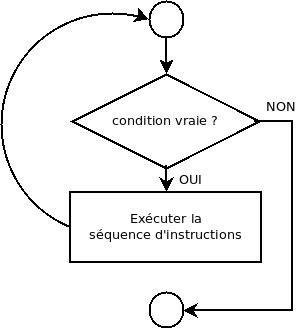
\includegraphics[width=0.5\textwidth]{image/boucle-tq}
		\caption{Ordinogramme de la boucle "tant-que"}
		\label{fig:boucle-tq}
	\end{figure}
\end{frame}

\subsubsection{«~faire – jusqu'à ce que~»}

\begin{frame}{«~faire – jusqu'à ce que~»}
	Cette structure est très proche du «~tant que~» 
	à deux différences près :
	
	\begin{enumerate}
		\item {
			Le test est fait à la fin et pas au début. La tâche est donc toujours
			exécutée au moins une fois. }
		\item {
			On donne la condition pour arrêter et pas pour continuer; il
			s'agit d'une différence mineure.}
	\end{enumerate}

	\bigskip
	
	\cadre{
		\begin{pseudo}
		\Repeat
			\Stmt séquence d’instructions à exécuter
		\Until{condition}
		\end{pseudo}
	}
\end{frame}

\begin{frame}{«~faire – jusqu'à ce que~»}
	\begin{itemize}
		\item 
			la séquence d’instructions comprise entre
			\code{faire} et \code{jusqu'a ce que} 
			contienne au moins une instruction qui modifie la condition de
			telle manière qu’elle puisse devenir \textbf{vraie} à un moment donné
			pour arrêter l'itération. 
	\end{itemize}
\end{frame}

\begin{frame}{«~faire – jusqu'à ce que~»}
	\begin{figure}[h]
	\centering
	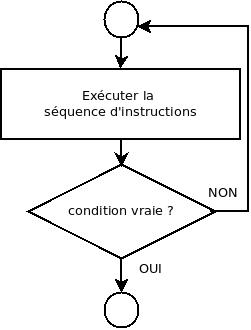
\includegraphics[width=0.4\textwidth]{image/boucle-faire}
	\caption{Ordinogramme de la boucle "faire – jusqu'à ce que"}
	\label{fig:boucle-faire}
	\end{figure}
\end{frame}

\subsubsection{«~pour~»}

\begin{frame}{«~pour~»}
	\begin{itemize}
		\item
		Ici, on va plutôt indiquer \textbf{combien de fois} la tâche doit être
		répétée. 
		\item
		Cela se fait au travers d'une
		\textbf{variable de contrôle} dont la valeur va évoluer à partir
		d'une valeur de départ jusqu'à une
		valeur finale.
	\end{itemize}
\end{frame}

\begin{frame}{«~pour~»}
	\cadre{
		\begin{pseudo}
		\For{variable \K{de} début \K{à} fin [\K{par} pas]}
			\Stmt séquence d’instructions à exécuter
		\EndFor
		\end{pseudo}
	}

	\begin{itemize}
		\item
		Dans ce type de structure, \code{debut}, \code{fin} et \code{pas}
		peuvent être des constantes, des variables ou des expressions (le plus
		souvent à valeurs entières mais on admettra parfois des réels). 
		\item
		Le \code{pas} est facultatif, et généralement omis (dans ce cas, sa valeur 
		par défaut est 1). 
		\item
		Ce pas est parfois négatif, dans le cas
		d'un compte à rebours, par exemple
		\code{pour n de 10 a 1 par -1}.
	\end{itemize}
\end{frame}

\begin{frame}{«~pour~»}
	\begin{itemize}
		\item
		Quand le \code{pas} est positif, la boucle s'arrête
		lorsque la variable dépasse la valeur de \code{fin}.
		\item
		Par contre, avec
		un \code{pas} négatif, la boucle s'arrête lorsque la
		variable prend une valeur plus petite que la valeur de \code{fin}
	\end{itemize}
\end{frame}

\begin{frame}{«~pour~»}
	\begin{figure}[h]
		\centering
		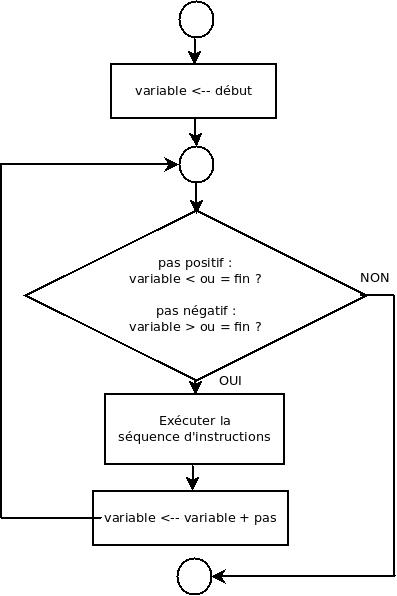
\includegraphics[width=0.4\textwidth]{image/boucle-pour}
		\caption{Ordinogramme de la boucle "pour"}
		\label{fig:boucle-pour}
		\end{figure}
\end{frame}

\begin{frame}{Attention}
	\begin{itemize}
		\item
		On considérera
		qu’au cas (à éviter) où \code{debut} est strictement supérieur à
		\code{fin} et le \code{pas} est positif, la séquence d’instructions
		n’est jamais exécutée (mais ce n’est pas le cas dans tous les langages
		de programmation !). 
		\item
		Idem si \code{debut} est strictement inférieur à
		\code{fin} mais avec un \code{pas} négatif.
		\item
		Attention de ne pas modifier dans la séquence d’instructions une des
		variables de contrôle \code{debut}, \code{fin} ou \code{pas} !
	\end{itemize}
\end{frame}

\begin{frame}{Attention}
	\begin{itemize}
		\item
		Il est aussi fortement déconseillé de modifier «~manuellement~» la
		\code{variable} de contrôle au sein de la boucle
		\code{pour}. Il ne faut pas l’initialiser en début de boucle,
		et ne pas s’occuper de sa modification, l’instruction 
		\code{variable} $\leftarrow$ \code{variable} + \code{pas} 
		étant automatique et implicite à chaque étape de la
		boucle.
		\item
		Il est aussi déconseillé d’utiliser \code{variable} à la
		sortie de la structure \code{pour} sans lui affecter une
		nouvelle valeur (son contenu pouvant varier selon le langage de
		programmation).
	\end{itemize}
\end{frame}


\begin{frame}{Exemples~}
	\cadre{
	\begin{pseudo}
	\Stmt \K{pour} i \K{de} 0 \K{à} 2 \K{faire} \RComment La boucle est exécutée 3 fois.
	\Stmt \K{pour} i \K{de} 2 \K{à} 0 \K{faire} \RComment La boucle n'est pas exécutée.
	\Stmt \K{pour} i \K{de} 1 \K{à} 10 \K{par} -1 \K{faire} \RComment La boucle n'est pas exécutée.
	\Stmt \K{pour} i \K{de} 1 \K{à} 1 \K{par} 5 \K{faire} \RComment La boucle est exécutée 1 fois.
	\end{pseudo}
	}
\end{frame}	

\subsection{Quel type de boucle choisir ?}

\begin{frame}{Quelle boucle choisir ?}
	\begin{itemize}
		\item
		En pratique, il est possible d’utiliser systématiquement la boucle 
		\code{tant que} qui peut s’adapter à toutes les situations. 
		\item
		Cependant, il est plus clair d’utiliser la boucle \code{pour} 
		dans les cas où le nombre d’itérations est fixé et connu à l’avance 
		\item
		La boucle \code{faire} convient quant à elle
		dans les cas où le contenu de la boucle doit être parcouru au moins une
		fois, 
		
		alors que dans \code{tant que}, 
		le nombre de parcours peut être nul si la condition initiale est fausse. 
	\end{itemize}
\end{frame}

\begin{frame}{Quelle boucle choisir ?}
	\begin{figure}[h]
	\centering
	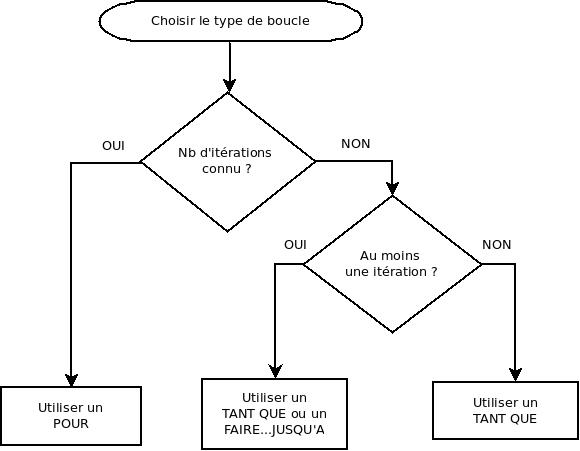
\includegraphics[width=0.7\textwidth]{image/boucle-choixtype}
	\caption{Quel type de boucle choisir ?}
	\label{fig:boucle-choix}
	\end{figure}
\end{frame}
	
\subsection{Exemples}

\subsubsection{Exemple 1 -- Compter de 1 à 10}

\begin{frame}{Compter de 1 à 10}
	Imaginons qu'on veuille afficher tous les nombres de 1 à 10. 
	
	On va évidemment \textbf{rejeter} cette première solution :

	\cadre{
	\begin{pseudo}
	\LComment Affiche les nombres de 1 à 10.
	\Module{compterJusque10}{}{} \RComment une mauvaise solution !
	\Write 1
	\Write 2
	\Write 3
	\Write 4
	\Write 5
	\Write 6
	\Write 7
	\Write 8
	\Write 9
	\Write 10
	\EndModule
	\end{pseudo}
	}
\end{frame}

\begin{frame}{Compter de 1 à 10}
	\begin{itemize}
	\item
	Non seulement c'est long à écrire 
	(imaginer l'algorithme pour afficher les nombres de 1 à 10000 !) 
	mais c'est très peu souple.
	\item
	Cela ne fonctionne que pour 10 : il faut modifier l'algorithme pour
	un autre comptage.
	\item
	La boucle va nous permettre
	d'obtenir un algorithme qui s'adapte
	à la limite du décompte.
	\end{itemize}
\end{frame}
	
\begin{frame}{Compter de 1 à 10}
	Posons-nous les bonnes questions pour déterminer la boucle :

	\begin{itemize}
	\item 
		Quelle est la tâche à répéter ? Afficher un nombre.
	\item 
		Comment savoir si on continue ? On arrête quand «~10~» est affiché.
	\item 
		Comment afficher à chaque fois un nombre différent ? 
		Au travers d'une variable qui prendra toutes les valeurs de 1 à 10. 
		Il faut donc ajouter dans le corps de la
		boucle une incrémentation de la variable
	\end{itemize}
\end{frame}

\begin{frame}{Compter de 1 à 10}
	Ce qui donne :

	\cadre{
	\begin{pseudo}
	\LComment A les nombres de 1 à 10.
	\Module{compterJusque10}{}{} \RComment version avec tant que
		\Decl nb : entier
		\Let nb \Gets 1 \RComment c'est le premier nombre à afficher
		\While{nb $\leq$ 10} \RComment tant que le nb à afficher est toujours bon
			\Write nb \RComment on affiche la valeur de la variable nb
			\Let nb \Gets nb + 1 \RComment on passe au nombre suivant
		\EndWhile
	\EndModule
	\end{pseudo}
	}
\end{frame}

\begin{frame}{Compter de 1 à 10}
	Mais ici, on pourrait aussi l'écrire avec un «~pour~» vu qu'on
	connait exactement le nombre d'exécutions de la boucle (10). 
	
	\medskip
	
	La variable de contrôle va évoluer de 1 à 10 ce qui tombe bien car
	c'est justement le nombre à afficher à chaque fois.
	
	\medskip

	\cadre{
	\begin{pseudo}
	\LComment Affiche les nombres de 1 à 10.
	\Module{compterJusque10}{}{} \RComment version avec pour
		\Decl nb : entier
		\For{nb \K{de} 1 \K{à} 10} \RComment par défaut le pas est de 1
			\Write nb 
		\EndFor
	\EndModule
	\end{pseudo}
	}
\end{frame}

\subsubsection{Exemple 2 -- Compter de 1 à beaucoup}

\begin{frame}{Compter de 1 à beaucoup}
	Dans l'exercice précédent, on a
	affirmé que la boucle pouvait s'adapter à la limite du
	décompte. Montrons-le ! 
	
	\bigskip
	
	Supposons qu'on veuille
	afficher les nombres de 1 à $n$ où $n$ est une valeur 
	donnée par l'utilisateur.

	\bigskip

	Rien de plus simple, il suffit de lire cette
	valeur au début et de l'utiliser comme limite de boucle
\end{frame}

\begin{frame}{Compter de 1 à beaucoup}
	\cadre{
	\begin{pseudo}
	\LComment Lit un nombre et affiche les nombres de 1 à ce nombre.
	\Module{afficherN}{}{} 
		\Decl nb, n : entier
		\Read n
		\For{nb \K{de} 1 \K{à} n} 
			\Write nb 
		\EndFor
	\EndModule
	\end{pseudo}
	}
\end{frame}

\begin{frame}{Compter de 1 à beaucoup}
	Que se passe-t-il si l'utilisateur entre une valeur négative ?
	
	\bigskip
	
	Comment améliorer le code pour que le programme
	le signale à l'utilisateur ?
\end{frame}

\subsubsection{Exemple 3 -- Afficher les nombres pairs}

\begin{frame}{Afficher les nombres pairs}
	Cette fois-ci on affiche uniquement les nombres 
	\textbf{pairs} jusqu'à la limite $n$.
	
	\bigskip
	
	\textbf{Exemple} : 
	les nombres pairs de $1$ à $10$ sont : $2$, $4$, $6$, $8$, $10$.
	
	\bigskip
	
	Notez que $n$ peut être impair. Si $n$ vaut $11$, 
	l'affichage est le même que pour $10$.

	\bigskip

	Est-ce qu'on peut utiliser un «~pour~» ? 
\end{frame}

\begin{frame}{Afficher les nombres pairs}
	Est-ce qu'on peut utiliser un «~pour~» ? 

	\bigskip
	
	Oui. De 1 à $n$, il y a exactement «~$n$ DIV $2$~» nombres à afficher. 
	
	\bigskip
	
	La difficulté vient du lien à faire entre la variable de
	contrôle et le nombre à afficher.
\end{frame}

\begin{frame}{Afficher les nombres pairs}

	\textbf{Solution 1} : 
	on garde le lien entre la variable de contrôle 
	et le nombre à afficher. 
	Dans ce cas, on commence à $2$ et le pas doit être de $2$.

	\bigskip
	
	\cadre{
	\begin{pseudo}
	\LComment Lit un nombre et affiche les nombres pairs jusqu'à ce nombre.
	\Module{afficherPair}{}{} 
		\Decl nb, n : entier
		\Read n
		\RComment limite des nombres à afficher
		\For{nb \K{de} 2 \K{à} n \K{par} 2} 
			\Write nb 
		\EndFor
	\EndModule
	\end{pseudo}
	}
\end{frame}

\begin{frame}{Afficher les nombres pairs}
	\textbf{Solution 2} : 
	la variable de contrôle compte simplement le nombre d'itérations.
	
	Alors il faut calculer le nombre à afficher en fonction de la variable
	de contrôle (ici le double de celle-ci convient)

	\bigskip
	
	\cadre{
	\begin{pseudo}
	\LComment Lit un nombre et affiche les nombres pairs jusqu'à ce nombre.
	\Module{afficherPair}{}{} 
		\Decl i, n : entier
		\Read n
		\RComment limite des nombres à afficher
		\For{i \K{de} 1 \K{à} n DIV 2} 
			\Write 2 * i 
		\EndFor
	\EndModule
	\end{pseudo}
	}
\end{frame}

\subsection{Exemple 4 -- Afficher les premiers nombres pairs}

\begin{frame}{Afficher les premiers nombres pairs}
	Voici un problème proche du précédent : 
	on affiche cette fois les $n$ premiers nombres pairs.
	
	\bigskip
	
	\textbf{Exemple} : 
	les $10$ premiers nombres pairs sont : $2$, $4$, $6$, $8$, $10$, $12$, $14$, $16$, $18$, $20$.
	
	\bigskip
	
	Il est plus simple de partir de la solution 2 de l'exemple précédent
	en changeant simplement la valeur finale de la boucle.
\end{frame}

\begin{frame}{Afficher les premiers nombres pairs}

		\cadre{
		\begin{pseudo}
		\LComment Lit un nombre et affiche ce nombre de nombres pairs.
		\Module{afficherPair}{}{} 
			\Decl i, n : entier
			\Read n
			\RComment le nombre de nombres à afficher
			\For{i \K{de} 1 \K{à} n} 
				\Write 2 * i 
			\EndFor
		\EndModule
		\end{pseudo}
		}
\end{frame}

\subsubsection{Exemple 5 -- Somme de nombres}

\begin{frame}{Somme de nombres}
	On veut pouvoir calculer (et retourner)
	la somme d'une série de nombres donnés par
	l'utilisateur. 
	
	\bigskip
	
	Il faut d'abord se
	demander comment l'utilisateur va pouvoir indiquer
	combien de nombres il faut additionner ou quand est-ce que le dernier
	nombre à additionner a été entré. 
	
	\bigskip
	
	Voyons quelques possibilités.
\end{frame}

\begin{frame}{Somme de nombres}
	\textbf{Variante 1}~: 
	
	L'utilisateur indique le nombre de termes au départ.
	
	\cadre{
	\begin{pseudo}
	\LComment Lit des valeurs entières et retourne la somme des valeurs lues.
	\Module{sommeNombres}{}{entier} \RComment Variante 1
		\Decl nbValeurs : entier \RComment nb de valeurs à additionner
		\Decl valeur : entier \RComment un des termes de l'addition
		\Decl somme : entier \RComment la somme
		\Decl i : entier \RComment itérateur
		\Let somme \Gets 0 \RComment la somme se construit petit à petit. 0 au départ
		\Read nbValeurs
		\For{i \K{de} 1 \K{à} nbValeurs} 
			\Read valeur
			\Let somme \Gets somme + valeur 
		\EndFor
		\Return somme
	\EndModule
	\end{pseudo}
	}
\end{frame}

\begin{frame}{Somme de nombres}
	\textbf{Variante 2}~: 
		
	Après chaque nombre, 
	on demande à l'utilisateur s'il y a encore un nombre à additionner.

	\bigskip
	
	Ici, il faut chercher une solution différente
	car on ne connait pas au départ le nombre de valeurs à additionner et
	donc le nombre d'exécution de la boucle. 
	
	\bigskip
	
	On va devoir passer à un
	«~tant que~» ou un «faire - jusqu'à ce que». 
	
	\bigskip
	
	On peut
	envisager de demander en fin de boucle si il reste
	encore un nombre à additionner. 
\end{frame}

\begin{frame}{Somme de nombres}
	\cadre{
	\begin{pseudo}
	\LComment Lit des valeurs entières et retourne la somme des valeurs lues.
	\Module{sommeNombres}{}{entier} \RComment Variante 2a
		\Decl encore : booléen \RComment est-ce qu'il reste encore une valeur à additionner ?
		\Decl valeur : entier \RComment un des termes de l'addition
		\Decl somme : entier \RComment la somme
		\Let somme \Gets 0
		\Repeat 
			\Read valeur
			\Let somme \Gets somme + valeur 
			\Read encore
		\Until{NON encore}
		\Return somme
	\EndModule
	\end{pseudo}
	}
\end{frame}

\begin{frame}{Somme de nombres}
	Avec cette solution, on additionne au moins une valeur. 
	
	\bigskip
	
	Si on veut pouvoir tenir compte du
	cas très particulier où l'utilisateur ne veut
	additionner aucune valeur, il faut utiliser un «~tant que~» et donc
	poser la question avant d'entrer dans la boucle.
\end{frame}

\begin{frame}{Somme de nombres}
	\cadre{
	\begin{pseudo}
	\LComment Lit des valeurs entières et retourne la somme des valeurs lues.
	\Module{sommeNombres}{}{entier} \RComment Variante 2b
		\Decl encore : booléen \RComment est-ce qu'il reste encore une valeur à additionner ?
		\Decl valeur : entier \RComment un des termes de l'addition
		\Decl somme : entier \RComment la somme
		\Let somme \Gets 0
		\Read encore
		\While{encore} 
			\Read valeur
			\Let somme \Gets somme + valeur 
			\Read encore
		\EndWhile
		\Return somme
	\EndModule
	\end{pseudo}
	}
\end{frame}

\begin{frame}{Somme de nombres}
	\textbf{Variante 3}~:
	
	L'utilisateur entre une valeur spéciale pour indiquer la fin. 
	On parle de valeur \textbf{sentinelle}. 
	
	\bigskip
	
	Ceci n'est possible que si cette valeur \textbf{sentinelle} ne peut pas être
	un terme valide de l'addition. 
	
	\bigskip
	
	Par exemple, si on veut
	additionner des nombres positifs uniquement, la valeur -1 peut servir
	de valeur sentinelle. 
	
	\bigskip
	
	Mais sans limite sur les nombres à additionner
	(positifs, négatifs ou nuls) il n'est pas possible de
	choisir une sentinelle.
\end{frame}

\begin{frame}{Somme de nombres}
	Ici, on se base sur la valeur entrée pour décider si on continue ou pas. 
	
	\bigskip
	
	Il faut donc \textbf{toujours} effectuer un test
	après une lecture de valeur. 
	
	\bigskip
	
	C'est pour cela
	qu'il faut effectuer une lecture avant et une autre à
	la fin de la boucle.

\end{frame}

\begin{frame}{Somme de nombres}
	\cadre{
	\begin{pseudo}
	\LComment Lit des valeurs entières et retourne la somme des valeurs lues.
	\Module{sommeNombres}{}{entier} \RComment Variante 3
		\Decl valeur : entier \RComment un des termes de l'addition
		\Decl somme : entier \RComment la somme
		\Let somme \Gets 0
		\Read valeur
		\While{valeur ${\geq}$ 0} 
			\Let somme \Gets somme + valeur 
			\Read valeur \RComment remarquer l'endroit où on lit une valeur.
		\EndWhile
		\Return somme
	\EndModule
	\end{pseudo}
	}
\end{frame}

\begin{frame}{Somme de nombres}
	\textbf{Réflexions}~: 
	\begin{itemize}
	\item
		Quelle valeur sentinelle prendrait-on 
		pour additionner une série de cotes d'interrogations ? 
		Une série de températures ?
	\item
		Dans les solutions 2 et 3 on lit une variable booléenne. 
		Comment un programmeur pourrait-il réaliser 
		cette instruction de façon pratique ?		
	\end{itemize}
\end{frame}

\subsubsection{Exemple 6~: Suite des nombres pairs}

\begin{frame}{Suite des nombres pairs}
	Écrire l'algorithme qui affiche les $n$ premiers termes
	de la suite: $2$, $4$, $6$\dots
	
	\bigskip
	
	Puisqu'on doit écrire plusieurs nombres et qu'on sait exactement combien,
	on se tournera tout naturellement vers une boucle \K{pour}.

	\bigskip
	
	Le cas le plus simple est lorsque le nombre à afficher à l'étape $i$
	peut être calculé en fonction de $i$ seulement.
	
\end{frame}

\begin{frame}{Suite des nombres pairs}
	\cadre{
	\begin{pseudo}
	\For{i de 1 à n}
		\Write $f(i)$
	\EndFor
	\end{pseudo}
	}
\end{frame}

\begin{frame}{Suite des nombres pairs}

	Dans ce cas, la fonction est $f(i)=2*i$
	(Si vous n'êtes pas convaincu, vérifiez qu'à l'étape $1$ on affiche $2$,
	à l'étape $2$ on affiche $4$ \dots)
	
	\bigskip

	\cadre{
	\begin{pseudo}
	\Module{nombrePair}{n\In: entier}{}
		\Decl i : entier
		\For{i de 1 à n}
			\Write 2 * i
		\EndFor
	\EndModule
	\end{pseudo}
	}
\end{frame}

\begin{frame}{Suite des nombres pairs}
	Parfois, il est difficile (voire impossible) de trouver $f(i)$.
	
	\bigskip
	
	On suivra alors une autre approche qui revient à calculer un nombre
	à afficher à partir du nombre précédemment affiché
	(ou, plus exactement, de calculer le suivant à partir du nombre
	qu'on vient d'afficher).
	La structure générale est alors

	\bigskip
	
	\cadre{
	\begin{pseudo}
	\Let nb \Gets \textit{\{1\up{ère} valeur à afficher\}}
	\For{i de 1 à n}
		\Write nb
		\Let nb \Gets \textit{\{calculer ici le nb suivant\}}
	\EndFor
	\end{pseudo}
	}
\end{frame}

\begin{frame}{Suite des nombres pairs}
	Dans l'exemple de la suite paire, le 1\up{er} nombre à afficher est $2$
	et le nombre suivant se calcule en ajoutant $2$ au nombre courant.

	\bigskip
	
	\cadre{
	\begin{pseudo}
	\Module{suite1}{n\In: entier}{}
		\Decl nb, i : entiers
		\Let nb \Gets 2
		\For{i de 1 à n}
			\Write nb
			\Let nb \Gets nb + 2
		\EndFor
	\EndModule
	\end{pseudo}
	}
\end{frame}

\begin{frame}{Suite des nombres pairs}
	On remarque que, lors du dernier passage dans la boucle,
	on calcule une valeur qui ne sera pas affichée.
	Cette petite perte de temps est dommage mais négligeable
	et permet de garder une structure claire et générale à la solution.

	\bigskip
	
	Dans certains cas,
	il n'est pas possible de déduire directement le nombre suivant
	en connaissant juste le nombre précédent.
	Prenons un exemple pour l'illustrer.
\end{frame}

\subsection{Exemple 7~: 3 pas en avant, 2 pas en arrière} 

\begin{frame}{3 pas en avant, 2 pas en arrière} 
	Écrire l'algorithme qui affiche les $n$ premiers termes
	de la suite: $1$, $2$, $3$, $4$, $3$, $2$, $3$, $4$, $5$, $4$, $3$\dots

	\bigskip
	
	Si on vient d'écrire, disons un $3$,
	impossible sans information supplémentaire,
	de connaitre le nombre suivant.
	
	\bigskip
	
	Il faudrait savoir si on est en phase d'avancement ou de recul
	et combien de pas il reste à faire dans cette direction.

	\bigskip
	
	Ajoutons des variables pour retenir l'\textbf{état} où on est.
\end{frame}

\begin{frame}{3 pas en avant, 2 pas en arrière} 
	\cadre{
	\begin{pseudo}
	\Module{suite3Avant2Arrière}{n\In: entier}{} 
		\Decl nb, nbPasRestants, direction, i : entiers
		\Let nb \Gets 1
		\Let nbPasRestants \Gets 3 \RComment 3 pas
		\Let direction \Gets 1 \RComment en avant
		\For{i de 1 à n}
			\Write nb
			\Let nb \Gets nb + direction \RComment faire un pas dans la bonne direction
			\Let nbPasRestants \Gets nbPasRestants - 1
			\If{nbPasRestants $=$ 0} \RComment il est temps de changer de direction
				\Let direction \Gets -direction
				\If{direction $=$ 1}
					\Let nbPasRestants \Gets 3 
				\Else 
					\Let nbPasRestants \Gets 2
				\EndIf
			\EndIf
		\EndFor
	\EndModule
	\end{pseudo}
	}
\end{frame}

\begin{frame}{3 pas en avant, 2 pas en arrière} 
	On obtient un algorithme plus long 
	mais qui respecte toujours le schéma vu.

	\bigskip
	
	\textbf{Un conseil}~: essayez de respecter ce schéma 
	et vous obtiendrez plus facilement un algorithme
	correct et lisible, également dans les cas particuliers.
\end{frame}
